% ЕМТ 2018, VII клас — точен LaTeX препис от официалните файлове в Klasirane.com.
% Условия: https://klasirane.com/api/competitions/EMT/All/2018/7%20%D0%BA%D0%BB/probs
% SHA-256 (условия): 9140adfd22b82e52373b9812c3084548e06fedfe75791c862c7bad986be96f5f
% Решения: https://klasirane.com/api/competitions/EMT/All/2018/7%20%D0%BA%D0%BB/sol
% SHA-256 (решения): 0c9d2b14e2f9dadcecf08d85896ae5655b4d3afe2dadf79331a760fd9dfedd92
% Точковите оценки, правописът и непълнотите са запазени от източника.

Задача 7.1. Даден е изразът $B=(5x-2)^2-2(x-4)(5x-2)+(x-4)^2$.

а) Намерете стойността на израза $B$ при $x=2017\dfrac{3}{4}.2018\dfrac{1}{4}-2017\dfrac{1}{4}.2018\dfrac{3}{4}$.

б) Докажете, че за всяка стойност на променливата $x$ стойността на израза $B$ е не по-малка от стойността на

$$A=\left|2^{33}-3^{22}\right|+\left|81^6-9^{11}\right|+\left|8^{11}-2^{32}\right|-\left|3^{24}-4^{16}\right|.$$

Решение: а) За намиране на $x=0,5$ — 2 т.

За намиране на стойността на $B=16$ — 3 т.

б) За намиране на $A=0$ — 2 т.

За преобразуване на $B$ във вид на квадрат на двучлен и доказване на неравенството — 3 т.

Задача 7.2. Лека кола и автобус тръгнали едновременно от град $A$ към град $B$ и се движили, без да спират. Скоростта на леката кола се отнасяла към скоростта на автобуса както $10:7$. Леката кола пристигнала в град $B$ в 10:50 ч., а автобуса – в 11:20 ч.

а) Намерете в колко часа те са тръгнали от град $A$.

б) Когато леката кола била изминала 80 % от разстоянието между двата града, тя срещнала камион, пътуващ за град $A$. Намерете в колко часа са се срещнали камионът и автобусът, ако скоростта на автобуса е била с 40 % по-голяма от скоростта на камиона.

Решение: а) Скоростта и времето за изминаване на определено разстояние са обратно пропорционални величини. Следователно времето за целия път на леката кола се отнася към времето на автобуса както $7:10$.

Ако $t_{\text{колата}}=7x$, а $t_{\text{автобуса}}=10x$, тогава $10x-7x=30$ min, т.е. $x=10$ min. — 1 точка

Леката кола е пътува $7.10=70$ min, автобусът – $10.10=100$ min. т.е. те са тръгнали от град $A$ в 9:40 ч. — 3 точки

б) Нека разстоянието между двата града е $S$. Нека колата е срещнала камиона в точка $C$ и в момента на срещата им автобусът се е намирал в т. $D$. Разстоянията, изминати от колата и автобуса за едно и също време е право пропорционално на скоростите им.

$$\dfrac{AC}{AD}=\dfrac{10}{7}\Rightarrow AD=\dfrac{7}{10}.\dfrac{4}{5}S=\dfrac{14}{25}S.$$

$$DC=\dfrac{4}{5}S-\dfrac{14}{25}S=\dfrac{6}{25}S.$$ — 2 точка

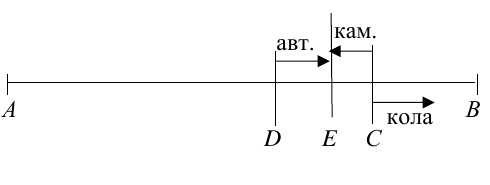
\includegraphics[max width=\textwidth, alt={Схема на движението между A и B с точките D, E и C}, center]{assets/7-2-solution-figure.png}

Разстоянията $DE$ и $CE$, изминати от камиона и автобуса до срещата им, са пропорционални на скоростите им, т.е. $\dfrac{DE}{CE}=\dfrac{140}{100}=\dfrac{7}{5}$. Ако $DE=7y$ и $CE=5y$, то

$$7y+5y=\dfrac{6}{25}S$$

и $y=\dfrac{6}{25}S.\dfrac{1}{12}=\dfrac{1}{50}S$. Тогава от $A$ до срещата автобусът е изминал разстоянието

$$AE=\dfrac{14}{25}S+\dfrac{7}{50}S=\dfrac{7}{10}S$$

за време, равно на $\dfrac{7}{10}.100=70$ min. Следователно срещата е станала в 10:50 ч.

Задача 7.3. Диагоналите на трапеца $ABCD$ се пресичат в точка $M$. Права, минаваща през точка $M$ и успоредна на бедрото $AD$, пресича голямата основа $AB$ на трапеца в точка $N$. Правата $CN$ пресича диагонала $BD$ в точка $O$.

а) Докажете, че лицето на триъгълника $BOC$ е равно на лицето на четириъгълника $ANOM$;

б) Ако лицата на триъгълниците $NOB$ и $COD$ са съответно равни на 16 cm$^2$ и 9 cm$^2$, намерете лицето на трапеца.

Решения: а) От $AB\parallel CD\Rightarrow S_{BOC}=S_{DNO}$.

$$S_{DNO}=S_{DNM}+S_{NMO}.$$ — 1 точка

От $MN\parallel AD\Rightarrow S_{DNM}=S_{ANM}$. — 1 точка

Тогава $S_{DNO}=S_{DNM}+S_{NMO}=S_{ANM}+S_{NMO}=S_{ANOM}$. — 2 точка

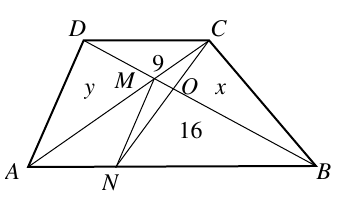
\includegraphics[max width=\textwidth, alt={Чертеж на трапеца ABCD с точките M, N и O}, center]{assets/7-3-solution-figure.png}

б) Нека $S_{BOC}=S_{DON}=S_{ANOM}=x$. От $\dfrac{S_{BOC}}{S_{COD}}=\dfrac{BO}{DO}=\dfrac{S_{BON}}{S_{DON}}$ получаваме $\dfrac{x}{9}=\dfrac{16}{x}$ и $x^2=144$, т.е. $x=12$ cm$^2$. — 2 точка

Нека $S_{AMD}=S_{BMC}=y$ cm$^2$ (от $AB\parallel CD$). Тогава $S_{DMC}=9-(y-12)=21-y$.

От $\dfrac{S_{AMB}}{S_{AMD}}=\dfrac{BM}{DM}=\dfrac{S_{BMC}}{S_{DMC}}$ получаваме $\dfrac{16+12}{y}=\dfrac{y}{21-y}$ и $y^2=28(21-y)$. — 2 точки

Решаваме уравнението $y^2+28y-588=0$, като го записваме във вида $(y+14)^2=784=28^2$ и намираме, че $y+14=28$, т.е. $y=14$. — 2 точки

Тогава лицето на трапеца $ABCD$ е

$$S=S_{BON}+S_{BOC}+S_{DOC}+S_{ANOM}+S_{AMD}=16+12+9+12+14$$

$=63$ cm$^2$. — 1 точки

Задача 7.4. Множеството $M$ се състои от числата от вида $3^k+1$, $4^k-1$, $5^k$ и $5^k+1$, където $k$ е естествено число, по-малко или равно на 50. Да се намери вероятността сборът на две случайно избрани числа от множеството $M$ да се дели на 6.

Решение:

$3^k+1\equiv4\pmod 6$; $4^k-1\equiv3\pmod 6$; $5^k\equiv1\pmod 6$ за $k=2p$ и $5^k\equiv5\pmod 6$ за $k=2p+1$;

$5^k+1\equiv2\pmod 6$ за $k=2p$ и $5^k+1\equiv0\pmod 6$ за $k=2p+1$. — 2 точка

Сбор на две числа, който се дели на 6, можем да получим по следните начини:

число от вида $3^k+1$ и число от вида $5^{2p}+1$: $50.25$ двойки — 2 точка

число от вида $5^{2p}$ и число от вида $5^{2p+1}$: $25.25$ двойки — 1 точка

две числа от вида $4^k-1$: $(50.49):2$ двойки — 1 точка

две числа от вида $5^{2p+1}+1$: $(25.24):2$ двойки — 1 точка

Общо благоприятни двойки: $25.(50+25+49+12)=25.136$ — 1 точка

Всички възможни двойки числа са $(200.199):2=100.199$ — 1 точки

Вероятността $p$ сборът на две числа да е кратен на 6 е $p=\dfrac{25.136}{100.199}=\dfrac{34}{199}$. — 1 точки
